\subsection{Data collection \& management}

We have developed a new platform that allows housing of mice in large arenas
(\textgreater 2m diameter), while manipulating and monitoring their behaviour
at high spatiotemporal resolution (Figure~\ref{fig:arena}).
%
We have openly shared software for supporting data acquistion
\citep{aeon_acquistion} and management \citep{aeon_mecha} in this arena.

\begin{figure}
    \begin{subfigure}{\textwidth}
        \centering
        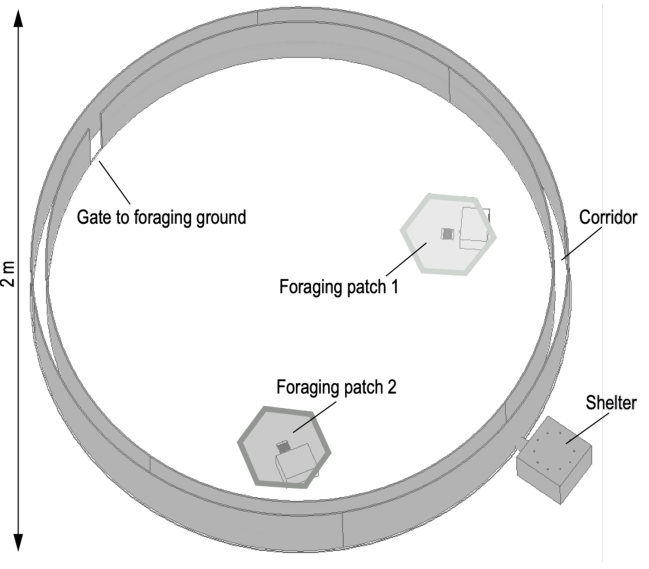
\includegraphics[width=4in]{figures/arena.png}
        \caption{}
    \end{subfigure}
    \par\bigskip
    \begin{subfigure}{\textwidth}
        \centering
        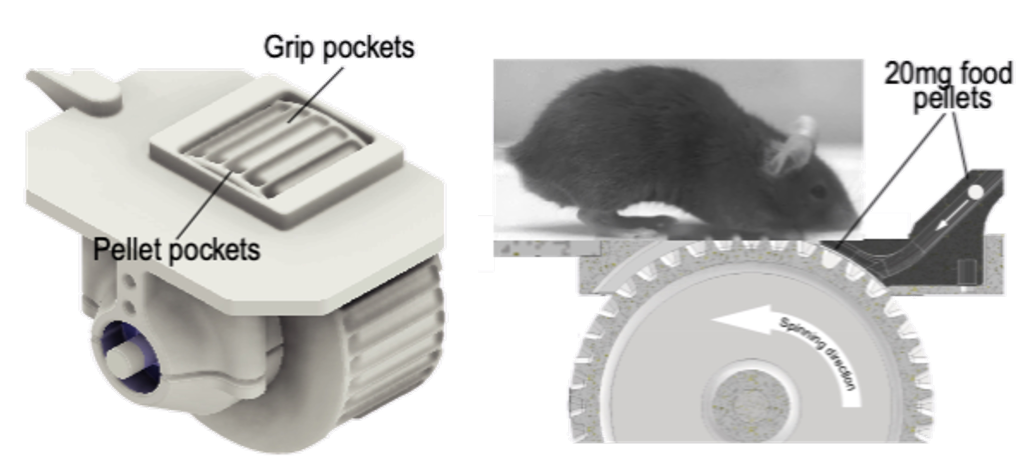
\includegraphics[width=4in]{figures/patch.png}
        \caption{}
    \end{subfigure}
    %
    \caption{Foraging arena (a) and feeder (b).
    %
    The floors of the arenas are tessellated to form honeycombs of modular
    hexagonal tiles (a), each of which can be equipped with a newly designed
    underground feeder (b).
    %
    Pellets are dispensed onto a foraging wheel once the mouse has spun it for
    a pre-defined programmable distance threshold using its forepaws (fictive
    digging).
    %
    The arena contains up to six scale-equipped nesting modules that allows
    housing of mice in the arena and weight monitoring.
    %
    Behavioural monitoring is achieved by an array of high-speed cameras (up to
    15), by which mouse location, mouse identity and body parts can be track in
    real time.
    %
    Long term monitoring of neural activity is performed using Neuropixels
    probes.
    %
    Using this platform we have collected several week long datasets both with
    single mouse and multiple mice.
    %
    These datasets capture a rich behavioural repertoire including a foraging
    behaviour,  social learning task, defensive and nesting behaviours.
    %
    }
    %
    \label{fig:arena}
\end{figure}
